\documentclass[]{article}
\usepackage{framed}
\usepackage{amsmath}
\usepackage{amssymb}
\usepackage{graphicx}
\usepackage{multicol}

\begin{document}
\subsection*{Chapter 6: Digraphs and Relations}
%-https://en.wikibooks.org/wiki/Set_Theory/Orderings

Definitions[edit]
Relations with certain properties that impose a notion of order on a set are known as order relations or simply orderings. For the following definitions, let R be a binary relation.

If R is reflexive and transitive, then it is known as a preorder.
If R is a preorder and also antisymmetric, then it is known as a partial order.
If R is a partial order and also total, then it is known as a total order or a linear order.

A set equipped with a preorder, partial order, or total order is known as a preordered set, partially ordered set (or poset), or totally ordered set (or linearly ordered set) respectively. An order relation is usually denoted by the symbol \le and an ordered set is denoted by the ordered pair ( S , \le ) where \le is the order relation on S.

A totally ordered subset of a partially ordered set is known as a chain. For this reason, any totally ordered set may sometimes be referred to as a chain.

Two elements a and b in a preordered (and thus in a partially or totally ordered) set are called comparable if either a \le b or b \le a. Note that while totality guarantees that every two elements in a totally ordered set are comparable, two elements in a pre or partially ordered set may not be so.

%=====================================================================================%
Equivalences[edit]
Another important type of relation is the equivalence relation. This is a relation R that is reflexive, symmetric, and transitive (or, simply a preorder that is also symmetric). When R is an equivalence relation, we usually denote it by \sim or \equiv. A set equipped with an equivalence relation is also known as a setoid.

If \sim is an equivalence relation on a set S, we define for an element s \in S the equivalence class of s as \{a \in S : a \sim s\}. This is usually denoted by [s]. The set of all equivalence classes of S is known as the quotient set of S by \sim, which we denote by S/\!\sim\ = \{[x] : x \in S\}.

A partition of a set S is a family of sets \mathfrak{S} such that \mathfrak{S} is pairwise disjoint and \bigcup \mathfrak{S} = S. The proof of the following theorems about equivalence relations are left to the reader.

Theorem: If S is a set and \sim is an equivalence relation on S, then S/\!\sim is a partition of S.

Theorem: Let S be a set and P a partition of S. Define a relation \star such that for a, b \in S, a \star b holds if and only if there exists a member of P which contains both a and b. Then, \star is an equivalence relation.

%==========================================================================================%

Chapter 1
D ` h d R l t`
Summary
Digraphs; Relations, using digraphs to illustrate relations, equivalence relations,
partial orders, relations and cartesian products.
%References: Epp Sections l0.l. 10.2, 10 3, 10.5 or B/1&:B Section 5.1.

\subsection*{Digraphs}
Some problems require that we dzrect the edges of a graph, from one endpoint to
the other, in order to express the relationship between the vertices A graph in
which every edge has a direction assigned to ir is called a \textit{\textbf{digraph}} (an abreviation
of directed graph). 

The directed edges are often called \textbf{arcs}.


\noindent\textbf{Example 1.1} Suppose we want to model a plan for traflic flow in part of a city,
where some streets allow trafiic flow in only one direction. 

For this model, a digraph would be appropriate, We would represent each road junction by a vertex; a one-way street from junction u to junction 1;, by an arc directed from u to UQ and a street allowing traffic flow in both directions between junctions rc and y, by two
arcs, one directed from x to y and the other from y to rv. 

An example is given in
Figure L17 where the direction of each arc is indicated by an arrow.
%-------- %
In a digraph we define directed paths and directed cycles as in graphs, but
with the added condition that arcs must be used in their correct direction, 

We say a digraph D is stongly corrected if for every pair of vertices x and y of D, there is a directed path from x to y and a directed path from y to x in D.
\begin{figure}[h!]
\centering
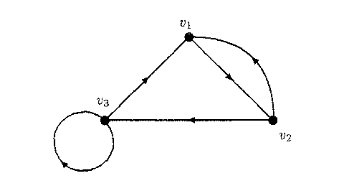
\includegraphics[width=0.7\linewidth]{./Digraph1}
\caption{}
\label{fig:Digraph1}
\end{figure}
%e 1.2: The relationship digraph of Example 1.3
Example 1.2 The digraph in Figure 1.1 contains a direcred path P = vamp; and
a directed cycle C : ugviug. lt is strongly connected.
Digraphs can be used to illustrate a variety of "one-way" relationships such as
predator-prey models in ecology, the scheduling of tasks in a manufacturing process.
family trees, flow diagrams for a computer program and many others.
\begin{figure}
\centering
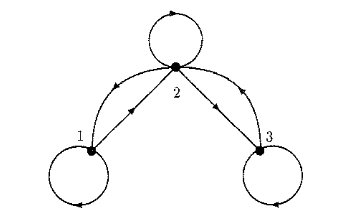
\includegraphics[width=0.7\linewidth]{./Digraph2}
\caption{}
\label{fig:Digraph2}
\end{figure}

